

\subsection{Objetivos:}
    \begin{itemize}
        \item Diseño de la lógica de control de un ascensor.
        \item Implementación y validación de dicho diseño en lenguaje VHDL.
        \item Simulación de cada entidad implementada para verificar su funcionamiento mediante un testbench en código VHDL.
        \item Sintetizado sobre la tarjeta SPARTAN-3 Starter Kit del laboratorio
    \end{itemize}
    
\subsection{Funcionamiento general del Ascensor y requisitos:}

\subsection{Placa Spartan-3 Starter Kit Board} \label{subsection:Spartan-3}
    
    Para la implementación de este proyecto y si realización sobre un soporte físico real se utilizará la placa Spartan-3 Starter Kit Board de Xilinx, que incluye la FPGA así como otros componentes que nos vendrán bien a la hora de simular el comportamiento del ascensor.

    En las figuras que se muestran a continuación se pueden ver la distribución de los componentes del Kit:

    \begin{figure}[H]
            \centering
            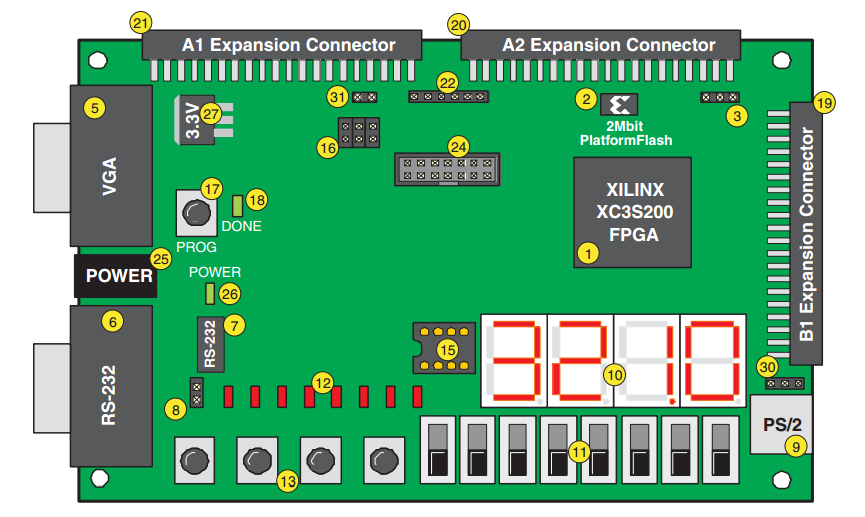
\includegraphics[width = 0.8\textwidth ]{Spartan3TopSide}
            \caption{Placa Spartan-3 (parte superior)}
            \label{fig:Spartan3TopSide}
    \end{figure}

    \begin{figure}[H]
            \centering
            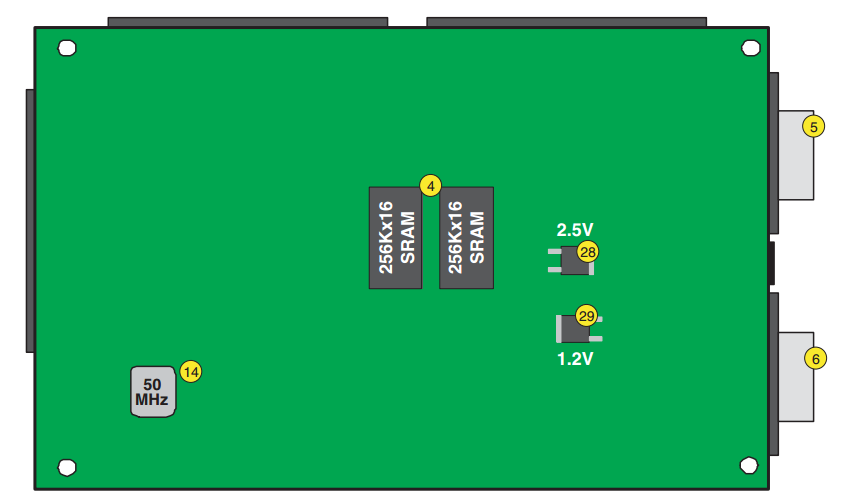
\includegraphics[width = 0.8\textwidth ]{Spartan3BottomSide}
            \caption{Placa Spartan-3 (parte inferior)}
            \label{fig:Spartan3BottomSide}
    \end{figure}

    Nos centraremos en los componentes más importantes que utilizaresmos para la realización de este proyecto:

    \begin{itemize}
        \item [1] Xilinx Spartan-3 XC3S200 FPGA  (encapsulado XC3S200FT256). Compuesta por 200000 puertas.
        \item [2] 2Mbit Xilinx XCF02S Platform Flash.
        \item [4] 1M-byte of Fast Asynchronous SRAM.
        \item [10] Cuatro displays LED de 7 segmentos.
        \item [11] Ocho interruptores.
        \item [12] Ocho salidas LED independientes.
        \item [13] Cuatro pulsadores.
        \item [14] Cristal osculador (CLK) de 50MHz.
        \item [18] LED indicador de que la FPGA ha sido configurada correctamente

    \end{itemize}

\subsection{Estructura de la memoria e información útil}

    En los siguientes apartados de la memoria se puede encontrar la explicación detallada del funcionamiento y codificación de la lógica del ascensor descrito, concretamente:
    \begin{itemize}
        \item Apartado \ref{section:DiagBloques}: Se detalla el funcionamiento interno de cada entidad o arquitectura así como su interfaz. A su vez se describe la relación entre las diferentes entidades
        \item Apartado \ref{section:Codigo}: Se adjunta la programación de cada entidad o arquitectura así como su correspondiente testbech.
        \item Apéndice \ref{app:codEntSal}: Se adjuntan las tablas donde se especifica la codificación que se ha utilizado para el funcionamiento interno del ascensor.
    \end{itemize}
    
    Todo el proyecto, tanto el documento en código \LaTeX\  como los ficheros VHDL se pueden encontrar en Github \faGithub\ en el siguiente enlace: https://github.com/enheragu/Elevator-VHDL
